% ============
% Dataset Construction
% ============
\section{Dataset Construction} \label{app:dataset-construction}

\begin{figure*}[t]
  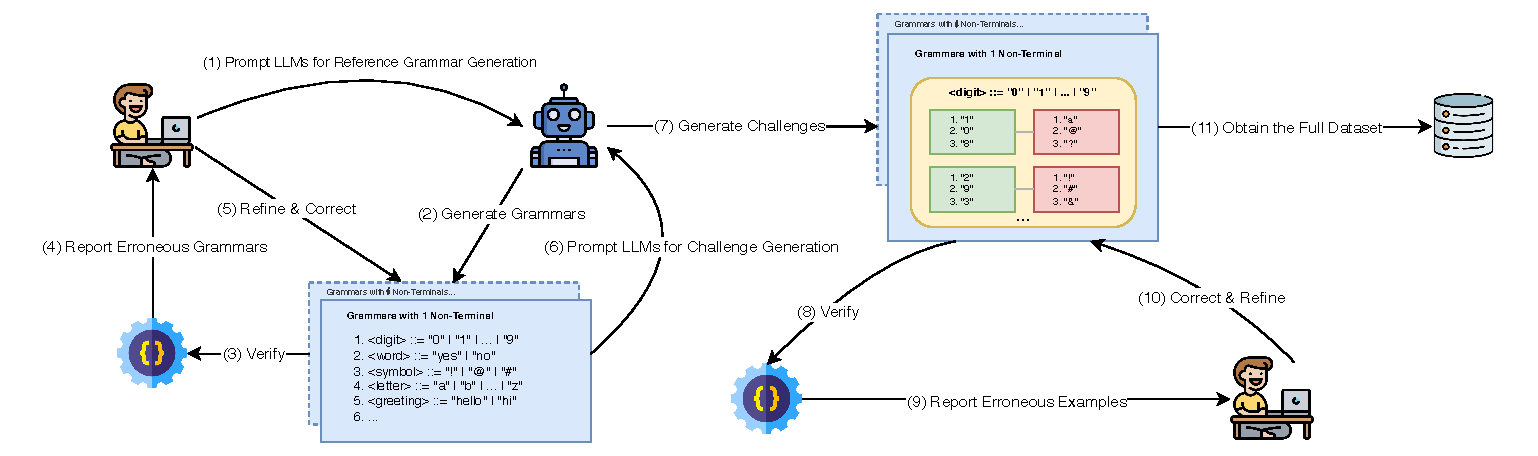
\includegraphics[width=\textwidth]{figures/dataset_construction.pdf}
  \caption{The Dataset Construction Process: (1) GPT-4o is prompted with Prompt Template~\ref{prompt:dc_generate_bnfs} to generate a set of reference grammars; (2) A set of reference grammars $\mathfrak{G^{ref}}=\bigcup^9_{k=1} \mathbb{G}^{ref}_{k}$ are generated by LLMs; (3) A BNF parser is used to check the correctness of each generated reference grammar; (4) Erroneous reference grammars are reported to humans; (5) Reported reference grammars are modified and corrected manually; (6) GPT-4o is prompted with Prompt Template~\ref{prompt:dc_generate_pexamples} and Prompt Template~\ref{prompt:dc_generate_nexamples} to generate challenges for each reference grammars; (7) Challenges are generated by LLMs, in which each challenge consists of 3 positive and 3 negative examples; (8) A BNF parser is used to verify whether positive and negative examples are accepted and rejected by their corresponding reference grammar respectively; (9) Erroneous challenges are reported to humans; (10) Reported challenges are corrected manually; (11) The final dataset consisting of 540 challenges are obtained.}
  \label{fig:dataset_construction}
\end{figure*}
To evaluate the capacity of LLMs in few-shot grammar generation, we present a dedicated dataset. We explain the details of the construction process in this section.

For clear explanation, let $\mathfrak{G}^{ref} = \bigcup_{k=1}^K \mathbb{G}^{ref}_{k}$ be a set of reference grammars, where $\mathbb{G}^{ref}_{k}$ is a set of reference grammars in which each reference grammar $G^{ref}_k$ having exactly $k$ non-terminals and thus its $|R| = k$. Each set of reference grammars $\mathbb{G}^{ref}_{k}=\{G^{ref}_{k,1}, G^{ref}_{k,2}, \dots, G^{ref}_{k,n}\}$ contains $n$ reference grammar with $k$ non-terminals. 

Initially, we constructed $\mathfrak{G}^{ref} = \bigcup_{k=1}^9 \mathbb{G}^{ref}_{k}$. For each number $k$, we prompted GPT-4o to produce $n=10$ reference grammars to yield $\mathbb{G}^{ref}_{k}=\{G^{ref}_{k,1}, G^{ref}_{k,2}, \dots, G^{ref}_{k,10}\}$, with the prompt template demonstrated in Prompt Template~\ref{prompt:dc_generate_bnfs}. In Prompt Template~\ref{prompt:dc_generate_bnfs}, $k$ means the placeholder of the number of non-terminals, and $n$ means the number of reference grammars needed to be produced. However, GPT-4o failed to consistently generate reference grammars in the correct syntax or with the correct number of non-terminals, especially as the number of non-terminals increased. To ensure that the generated reference grammars are syntactically correct and have the correct number of non-terminals, we used a BNF parser to do verification. It takes a $G^{ref}$ and checks whether $valid(G^{ref})$ is true and whether it has the required number of non-terminals. Any reference grammar that is not valid or has a wrong number of non-terminals were manually corrected. For duplicated reference grammars, we prompted GPT-4o to generate an alternative. This resulted in 90 reference grammars (i.e., $|\mathfrak{G}^{ref}| = |\bigcup_{k=1}^{9} \mathbb{G}^{ref}_{k}| = 90$), which are the reference grammars used to generate positive and negative examples subsequently.

For each reference grammar $G^{ref} \in \mathfrak{G}^{ref}$, we prompted GPT-4o to generate $6$ various challenges. For each challenge, GPT-4o is prompted by Prompt Template~\ref{prompt:dc_generate_pexamples} and Prompt Template~\ref{prompt:dc_generate_nexamples} to produce a set of $3$ positive examples ($\mathcal{P} \subseteq \mathcal{L}(G^{ref})$), and a set of three negative examples ($\mathcal{N} \cap \mathcal{L}(G^{ref}) = \emptyset$), respectively. In both Prompt Template~\ref{prompt:dc_generate_pexamples} and Prompt Template~\ref{prompt:dc_generate_nexamples}, $m$ means the number of examples needed to be generated, and \textit{reference\_grammar} means the given reference grammar by which the generated examples should be accepted or rejected. However, we observed that GPT-4o frequently failed to produce valid positive and negative examples, leading to either $\mathcal{P} \not\subseteq \mathcal{L}_(G^{ref})$ or $\mathcal{N} \cap \mathcal{L}_(G^{ref}) \neq \emptyset$, or both. The number of failures tends to increase as the number of non-terminals of $G^{ref}$ increases. To ensure the correctness of the generated challenges, we used a BNF parser to verify whether all given positive examples and negative examples can be accepted and rejected, respectively, by their corresponding $G^{ref}$. Erroneous positive and negative examples were manually corrected. Ultimately, we obtained a dataset consisting of a total of 540 challenges.

We visually summarize the dataset construction procedure in Figure~\ref{fig:dataset_construction}.

% ============
% Metrics
% ============
\section{Grammar Quality Metrics}
\label{appendix:grammar_quality_metrics}
This section covers the formal definitions of the grammar quality metrics. 


First define $\Pi_\mathcal{P} \subseteq \Pi$ to be the set of production rules that are used in the left-most derivations of all positive examples in $\mathcal{P}$. That is, the set of rules in $\Pi$ which occur in a sequence of rules $S \rightarrow \alpha_1 \rightarrow \ldots \rightarrow \alpha_n \rightarrow p $ where $p \in \mathcal{P}$, and all rules expand the left-most non-terminal in $\alpha_1, \ldots, \alpha_n$. 


% First define a $\mathrm{ProdUsed}$ function for measuring the number of production rules used during derivation for a grammar $\mathcal{G}$: 
% \[
% \mathrm{ProdUsed}(\mathcal{E}^{\mathcal{G}}, \mathcal{P})
% \;=\;
% \Bigl|\{\,a \in R
% \;\bigm|\;
% S \overset{*}{\underset{a}{\Rightarrow}} p
% \}\Bigr|.
% \]
% where $p \in \mathcal{P}$ , and $S$ derives $p$ in zero or more steps using production rule $a \in R$. 

Let $\Pi^*$ be the production rules in $\guess$ and $\Pi^{ref}$ be the production rules in $\bnfref$. Let us define $\diff(\bnfref,\guess) =  |\Pi^{ref}_\mathcal{P}| - |\Pi^*_\mathcal{P}|.$
%
%
The average difference in production rules used over the whole set of $k$ solved challenges, $C'$, is given by: 
$$
\diff^\diamond = \frac{1}{k} \sum_{i=1}^k \diff(\bnfref_i,\guess_i).
$$


% We define the difference of the number of used production rules between two grammars as:
% \[
% \mathrm{PUDiff}(\mathcal{E}^{\mathcal{G}_{(1)}},\mathcal{E}^{{\mathcal{G}}_{(2)}},\mathcal{P}) = \mathrm{PU_{(1)}} - \mathrm{PU_{(2)}}
% \]
% where $\mathrm{PU_{(1)}} = \mathrm{ProdUsed}(\mathcal{E}^{\mathcal{G}_{(1)}},\mathcal{P})$ and $\mathrm{PU_{\mathcal{G}^2}} = \mathrm{ProdUsed}(\mathcal{E}^{\mathcal{G}_{(2)}},\mathcal{P})$ to indicate the difference of the number of used production rules between $\mathcal{G}_{(1)}$ and $\mathcal{G}_{(2)}$.

% The $\diff_{avg}$ is given as:
% \begin{align*}
%     \mathrm{\diff_{avg}}(C) = \frac{1}{N} \sum_{i=1}^N \mathrm{PUDiff}(\mathcal{E}^{\mathcal{G}_{ref}}_i,\mathcal{E}^{\mathcal{G}_{llm}}_i,\mathcal{P}_i).
% \end{align*}
% to measure the average difference of used production rules between reference and generated grammars.

% Let $\mathrm{PUDiff}^{(1)}_{(2)}$ be $\mathrm{PUDiff}(\mathcal{E}^{\mathcal{G}_{(1)}},\mathcal{E}^{\mathcal{G}_{(2)}},\mathcal{P})$ and $\mathrm{ProdUsed^{(1)}}$ be $\mathrm{ProdUsed(\mathcal{E}^{\mathcal{G}_{(1)}},\mathcal{P})}$. 

\noindent We define two indicator functions, which indicate when a grammar uses substantially fewer rules than the reference grammar, and substantially more rules than the reference grammar:
% \begin{align*}
% \mathbb{I}_{OF}(\mathcal{E}^{\mathcal{G}_{(1)}},\mathcal{E}^{\mathcal{G}_{(2)}},\mathcal{P}) &= 
% \begin{cases}
% 1 & \text{if } (\mathrm{PUDiff}^{(1)}_{(2)} \\ & \quad > \frac{\mathrm{ProdUsed^{(1)}}}{2}) \\
% 0 & \text{otherwise.}
% \end{cases}
% \end{align*}
\begin{align*}
\mathbb{I}_{OF}(\bnfref, \guess,\mathcal{P}) &= 
\begin{cases}
1 & \text{if } |\Pi^{ref}_\mathcal{P}| - |\Pi^*_\mathcal{P}|
\\ & \quad
> \frac{|\Pi^{ref}_\mathcal{P}|}{2} \\
0 & \text{otherwise.}
\end{cases}
\end{align*}
\begin{align*}
\mathbb{I}_{OG}(\bnfref, \guess,\mathcal{P}) &= 
\begin{cases}
1 & \text{if } |\Pi^{ref}_\mathcal{P}| - |\Pi^*_\mathcal{P}|
\\ & \quad
< -\frac{|\Pi^{ref}_\mathcal{P}|}{2} \\
0 & \text{otherwise.}
\end{cases}
\end{align*}



The metric to estimate whether the generated grammars overfit the examples, is then given by
$$
 \of(C') = \frac{1}{k}\sum_{i=1}^{k} \mathbb{I}_{OF}(\bnfref_i,\guess_i, \mathcal{P}_i).
$$


% We also define an indicator function:
% \begin{align*}
% \mathbb{I}_{OG}(\mathcal{E}^{\mathcal{G}_{(1)}},\mathcal{E}^{\mathcal{G}_{(2)}},\mathcal{P}) &= 
% \begin{cases}
% 1 & \text{if } (\mathrm{PUDiff}^{(1)}_{(2)} \\ &\quad < -\frac{\mathrm{ProdUsed^{(1)}}}{2}) \\
% 0 & \text{otherwise.}
% \end{cases}
% \end{align*}
The metric to estimate whether the generated grammars overgeneralize the examples, $\og$, is given as:
\begin{align*}
    \og(C') = \frac{1}{k}\sum_{i=1}^{k}  \mathbb{I}_{OG}(\bnfref_i, \guess_i, \mathcal{P}_i).
\end{align*}

In addition, the $\tu$ metric, for a given challenge, to measure the percentage of $|\Pi^*|$ taken up by $|\Pi^*_\mathcal{P}|$, indicating the utility of $\guess$, is given as:
$$\tu(G^*,\mathcal{P}) = \frac{|\Pi^*_\mathcal{P}|}{|\Pi^*|}$$ for which lower $TU$ indicates a bunch of irrelevant or nonsensical production rules of $\guess$ while higher $TU$ indicates the opposite. The average utility over $C'$ is given by:$$\tu^\diamond = \frac{1}{k}\sum_{i=1}^{k} \tu(G^*_i,\mathcal{P})$$

% ============
% Direct Prompting
% ============
\section{Direct Prompting}
\label{appendix:DP}

For the DP approach, Prompt Template~\ref{prompt:direct_prompting} is used to prompt LLMs to directly generate a grammar with a given set of positive and negative examples. In Prompt Template~\ref{prompt:direct_prompting}, \textit{positive\_examples} and \textit{negative\_examples} are placeholders for a set of positive and negative examples. In addition, it also specifies a list of requirements LLMs should take care of and obey when generating grammars. 

% ============
% Optimization of BNF Parser for Providing LLM-Friendly Feedback
% ============
\section{Optimization of BNF Parser for Providing LLM-Friendly Feedback}
\label{appendix:OPF}

For the OPF approach, we use the same prompt template used in DP, as shown in Prompt Template~\ref{prompt:direct_prompting}, to prompt LLMs to generate an initial grammar. Then, Prompt Template~\ref{prompt:feedback_in_opf} is used in the iterations of the feedback loop to construct prompts from feedback offered by the BNF parser to LLMs. In Prompt Template~\ref{prompt:feedback_in_opf}, \textit{positive\_examples} and \textit{negative\_examples} are the placeholders for a set of positive and negative examples, \textit{bnf\_grammar} means the previously generated erroneous grammar, and \textit{parser\_feedback} is the placeholder for feedback provided from the BNF parser.


Furthermore, for each feedback given by the BNF parser, in addition to giving essential feedback such as notifying the line number for the place the error occurs, we optimize the BNF parser to also provide LLM-friendly feedback to LLMs, such as the possible reasons for the error or ways to fix it. We have shown some of them in Parser Feedback~\ref{feedback:invalid_rule} and Parser Feedback~\ref{feedback:lack_of_alts}.


In addition, OPF includes a parameter called \textit{max\_turns}, which specifies the maximum number of feedback iterations. If an LLM can generate a valid grammar based on earlier feedback, the algorithm stops early; otherwise, it continues until reaching the specified maximum.

Moreover, it is worth noting that this approach does not aim to follow every component of Reflexion or Self-Refine strictly. For instance, it does not maintain a long-term context or external memory. Instead, it uses only the most recent feedback in each turn to guide self-refinement. Concretely, in each feedback iteration, an LLM is provided with the previously generated erroneous grammar, corresponding positive and negative examples, and the latest feedback, to produce revised grammars. Therefore, since, in each iteration, an LLM may produce similar and even the same grammar as the previous ones, especially when they fail to fix the previous errors leading to the same feedback provided by the parser, we set the temperature to 0.3 to expect to enable LLMs to generate more diverse grammars even for encountering the same feedback, to optimize the performance. This approach highlights the optimization from the perspective of the parser to provide more LLM-friendly feedback. However, due to limited space and the trivial-yet-complex optimization process, for the details of the optimization of the BNF parser, please refer to our source code and the comments.

% We have also demonstrated the pseudocode of OPF in Algorithm~\ref{algo:opf}, in which $\mathcal{P}$ and  $\mathcal{N}$ mean a set of positive and negative examples respectively, $max\_turns$ means the maximum turns for the feedback loop, and $LLM$ is an LLM to generate grammars. 

% \begin{algorithm*}[t]
% \caption{OPF}
% \label{algo:opf}
% \begin{algorithmic}[1]
% \Procedure{GenerateGrammar}{$\mathcal{P}, \mathcal{N}, max\_turns, LLM$}
%     \State $prompt \gets \textsc{PromptGenerator}$ \Comment{Use prompt template from Prompt~\ref{prompt:direct_prompting}}
%     \State $\mathcal{G} \gets LLM(prompt)$ \Comment{Use LLM to get an initial grammar}
%     \For{$i \gets 1$ \textbf{to} \textit{max\_turns}}
%         \State $parsable, error \gets \textsc{Parse}(\mathcal{G})$ \Comment{Parse the given grammar using the BNF parser}
%         \If{not $parsable$}
%             \State $feedback \gets \textsc{FeedBackPromptGenerator}$ \Comment{Use prompt template from Prompt~\ref{prompt:feedback_in_opf}} 
%             \State $\mathcal{G} \gets LLM(feedback)$ \Comment{Use LLM to get a new grammar}
%         \EndIf
%     \EndFor
%     \Return $\mathcal{G}$
% \EndProcedure
% \end{algorithmic}
% \end{algorithm*}

% ============
% LLM-Driven Heuristic Mutation Genetic Algorithm
% ============
\section{LLM-Driven Hybrid Genetic Algorithm}
\label{appendix:LDHGA}

The pseudocode of \NAME is presented in Algorithm~\ref{algo:ldhga}, with detailed descriptions of its primary functions including $\mathrm{Fitness}$, $\mathrm{Select}$, $\mathrm{Cross}$, and $\mathrm{Mutate}$ provided in Section~\ref{sec:ldhm_ga}. In Algorithm~\ref{algo:ldhga}, we note $\mathrm{Fitness}$ function as \textsc{Fitness}, $\mathrm{Select}$ function as \textsc{Select}, $\mathrm{Cross}$ function as \textsc{Cross}, and $\mathrm{Mutate}$ function as \textsc{Mutate}.

As shown in Algorithm~\ref{algo:ldhga}, it takes seven parameters: $\mathcal{P}$ and $\mathcal{N}$ means a set of positive and negative examples respectively, $k$ indicates \emph{population size}, $g$ represents \emph{generations} which means the number of iterations of evolution, $\rho$ means the \emph{crossover rate}, $\mu$ means the \emph{mutation rate}, and $LLM$ means an LLM which takes a prompt and returns a response. In addition, \textsc{PromptGenerator} means to generate a prompt from the prompt template shown in Prompt Template~\ref{prompt:direct_prompting}. \textsc{MaxFitnessScore} is a constant indicating the highest fitness score any candidate grammar can achieve and due to each challenge in the constructed dataset only having 3 positive and 3 negative examples, the highest fitness score is 6. We thus set \textsc{MaxFitnessScore} to 6.

In addition, for \textit{LLMMut}, we have shown the prompt template used to prompt LLMs to mutate a given grammar in Prompt Template~\ref{prompt:llm_driven_mutation}, in which \textit{bnf\_grammar} means the placeholder for a candidate grammar while \textit{positive\_examples} and \textit{negative\_examples} means a set of positive and negative examples respectively.

\begin{algorithm*}[h]
\caption{\NAME}
\label{algo:ldhga}
\begin{algorithmic}[1]
\Procedure{GenerateGrammar}{$\mathcal{P}, \mathcal{N}, k, g, \rho, \mu, LLM$}
    \State $population \gets []$ \Comment{Initialize population as an empty list}
    \State $G^*.best \gets \texttt{null}$ \Comment{Keep track of overall best grammar}
    \State $fitness.best \gets -1$ \Comment{Track highest fitness found so far}
    \For{$i \gets 1$ \textbf{to} $k$}
        \State $prompt \gets \textsc{PromptGenerator}$ \Comment{Use prompt template from Prompt Template~\ref{prompt:direct_prompting}}
        \State $G^* \gets LLM(prompt)$ \Comment{Use LLM to get an initial candidate}
        \State $score \gets \textsc{Fitness}(G^*, \mathcal{P}, \mathcal{N})$ \Comment{Compute fitness}
        \If{$score = \textsc{MaxFitnessScore}$} 
            \State \Return $G^*$ \Comment{Return early if perfect score is achieved}
        \EndIf
        \State $population \gets population \parallel [G^*]$ \Comment{Add candidate to population}
    \EndFor
    \For{$i \gets 1$ \textbf{to} $g$}
        \State $fitnessScores \gets []$ 
        \For{$G^* \in population$}
            \State $score \gets \textsc{Fitness}(G^*, \mathcal{P}, \mathcal{N})$
            \State $fitnessScores \gets fitnessScores \parallel [(score, G^*)]$ \Comment{Add a tuple of score and grammar}
            \If{$score > fitness.best$}
                \State $fitness.best \gets score$
                \State $G^*.best \gets G^*$
            \EndIf
        \EndFor
        \If{$fitness.best = \textsc{MaxFitnessScore}$}
                \State \Return $G^*.best$ \Comment{Return the best grammar found} 
        \EndIf
        % \State \textsc{Sort}($fitnessScores$) \Comment{Sort by score in descending order}

        \State $\mathbb{G} = [G^* \mid (score, G^*) \in fitnessScores]$
        \State $S = [score \mid (score,G^*) \in fitnessScores]$
        \State $selected \gets \textsc{Select}(\mathbb{G},S)$
        \State $population.new \gets []$

        \While{$|population.new| < k$}
            \State $ G^*_a,G^*_b \gets \textsc{RandomChoice}(selected)$
            \State $G^* \gets \textsc{cross}(G^*_a,G^*_b, \rho)$
            \If{$\textsc{Uniform}(0,1) < \mu$}
                \State $G^* \gets \textsc{mutate}(G^* ,\mathcal{P}, \mathcal{N}, LLM)$
            \EndIf
            \State $population.new \gets population.new \parallel [G^*]$
        \EndWhile
        
        \State $population \gets population.new$ \Comment{Proceed to the next generation}
    \EndFor
    \Return $G^*.best$
\EndProcedure
\end{algorithmic}
\end{algorithm*}


\section{Additional Results}
\label{appendix:additional_results}
In addition to the results shown in Table~\ref{tab:results_for_all}, we have shown 7 more results and discussed them respectively in subsections~\ref{appendix:nonterminals_results},~\ref{appendix:prs_results},~\ref{appendix:fgi_results},~\ref{appendix:tu_results}, and~\ref{appendix:multiple_experiments}.

\subsection{Results for $C_1$, $C_2$, and $C_3$}
\label{appendix:nonterminals_results}
Table~\ref{tab:nonterminals_results} presents the results categorized into three subsets: $C_1$, $C_2$, and $C_3$. The subset $C_1$ includes challenges where the reference grammars have $1\sim3$ non-terminals, $C_2$ are those with $4\sim6$ non-terminals, and $C_3$ consists of challenges with $7\sim9$ non-terminals. Therefore, it aims to demonstrate and analyze the performance of LLMs as the number of non-terminals increases.

As the results are shown in Table~\ref{tab:nonterminals_results}, as the number of non-terminals increases, both $\sx$ and $\se$ decrease across all LLMs. While DP and OPF exhibit suboptimal and unsatisfactory performance, \NAME consistently demonstrates and contributes substantial improvements across most LLMs, even as the number of non-terminals increases. For example, in the case of \textit{GPT-4o}, \NAME increases the $\se$ by 21\% compared to DP and OPF on $C_3$. Similarly, with \textit{GPT-3.5-Turbo}, compared to DP and OPF, \NAME improves the $\se$ by 30\% and 28\% on $C_2$ and 20\% and 19\% on $C_3$, respectively.

\subsection{Results for $P_1$, $P_2$, and $P_3$}
\label{appendix:prs_results}
Table~\ref{tab:prs_results} demonstrates the results grouped into three subsets: $P_1$, $P_2$, and $P_3$. The subset $P_1$ consists of challenges where the reference grammars have $1\sim6$ production rules, $P_2$ includes those with $7\sim15$ production rules, and $P_3$ consists of challenges with the number of production rules greater than $16$. Therefore, it aims to show and analyze the performance of LLMs as the number of production rules increases. 

Similar to the results of $C_1$, $C_2$, and $C_3$, as the number of production rules increases, both $\sx$ and $\se$ decrease across all LLMs. Nevertheless, \NAME can still steadily improve both $\se$ and $\sx$, even as the number of production rules increases.

\subsection{Results for $\diff$, $\of$, and $\og$ Metrics}
\label{appendix:fgi_results}
To investigate whether LLMs generate grammars in an overfitted manner and whether \NAME improves performance through overfitting, as well as to examine whether LLMs and our method produce overly generalized grammars, we employed the three evaluation metrics: $\diff$, $\of$, $\og$. The results are presented in Table~\ref{tab:fgi_diff}, ~\ref{tab:fgi_of}, and~\ref{tab:fgi_og}, respectively. The notation “N/A” indicates inapplicability. Since these three metrics are only applicable when a grammar possesses correct semantics, “N/A” thus signifies that no grammar in the evaluation set exhibits correct semantics.

Through the $\diff$ metric, as shown in Tabel~\ref{tab:fgi_diff}, we observe that the number of production rules used in derivations of the generated grammars and the reference grammars does not differ significantly on average. However, as the number of production rules in the reference grammar increases, the $\diff^\diamond$ exhibits a slight upward trend. The $\diff^\diamond$ is almost always positive across most LLMs and methods, which indicates that, in most cases, the number of production rules used by the generated grammars is lower than that of the reference grammars.

Furthermore, Table~\ref{tab:fgi_of} presents the $\of$ metric. For some models, particularly \textit{GPT-3.5-Turbo}, an increasing number of production rules corresponds to a certain degree of overfitting. Nevertheless, on average, most LLMs do not exhibit significant overfitting. Additionally, we observe that in \NAME, the $\of$ metric does not show a significant difference compared to the baselines, indicating that \NAME does not improve performance through overfitting.

Additionally, we present the $\og$ metric in Table~\ref{tab:fgi_og}. We observed that, for some models, such as \textit{Qwen:72b-Instruct}, as the number of production rules in the reference grammar increases, they tend to generate overly generalized grammars. Nevertheless, on average, most LLMs do not tend to generate overgeneralized grammars.

\subsection{Results for $\tu$ Metrics}
\label{appendix:tu_results}
To investigate whether LLMs generate irrelevant production rules, we employ the $\tu$ metric. For example, given the challenge shown in Figure~\ref{fig:bnf_generation}, a generated grammar might be:

\vspace{1em}
\begin{minipage}{\linewidth}
\begin{verbatim}
<stmt> ::= <func> "(" <args> ")"
<args> ::= <expr> | <expr> "," <args>
<expr> ::= <char> | <number>
<func> ::= <char> <func> | <char>
<char> ::= "a" | ... | "z"
<number> ::= "0" | ... | "9"
<hello> ::= "hello"
<world> ::= "world"

\end{verbatim}
\end{minipage}
\vspace{1em}
in which:

\vspace{1em}
\begin{minipage}{\linewidth}
\begin{verbatim}
<hello> ::= "hello"
<world> ::= "world"

\end{verbatim}
\end{minipage} 
\vspace{1em}
are two irrelevant production rules.

As shown in Table~\ref{tab:fgi_tu}, on average, across both baselines and in \NAME, TU remains relatively high, indicating that LLMs do not tend to produce irrelevant production rules. However, as the number of production rules increases, $\tu$ shows a tendency of declination. Nevertheless, this does not imply that LLMs generate more irrelevant rules. Considering the results from $\og$, we think this decrease may more likely be attributable to the generated grammar becoming more generalized.

\subsection{Results for Robustness Evaluation}
\label{appendix:multiple_experiments}

Since \NAME requires setting the temperature greater than 0 which we set to 0.7, we repeated 5 independent experiments for both \textit{GPT-4o} and \textit{GPT-3.5-Turbo} to ensure the temperature does not affect the results significantly.

The results are demonstrated in Table~\ref{tab:5_times}, in which each row means the results of one experiment. The averages of syntax correctness of \textit{GPT-4o} and \textit{GPT-3.5-Turbo} are 95.8\% and 98.6\% and the standard deviations are 0.4\% and 0.49\%, respectively. The averages of semantic correctness of \textit{GPT-4o} and \textit{GPT-3.5-Turbo} are 93.2\% and 61.6\% and the standard deviations are 0.4\% and 0.49\%. Therefore, it indicates that although we set the temperature to 0.7 in \NAME, the fluctuation of both syntax correctness and semantic correctness are very slight and the performance across multiple experiments stays steady. Thus, the results demonstrated the robustness of our proposed method, \NAME.


% ===============
% Move prompts here for a better layout
% ===============

\begin{promptblock}{Generate a Grammar Directly with a Given Set Positive and Negative Examples}
\label{prompt:direct_prompting}
Given a set of positive and negative examples, generate the Backus–Naur Form (BNF) grammar that accepts all positive examples and rejects all negative examples.\\
1. Only generate the standard BNF grammar;\\
2. The generated BNF grammar MUST accept all positive examples and reject all negative examples;\\
3. Each terminal symbol MUST be quoted with double quotes and MUST NOT escape double quotes or pipeline in terminal symbols;\\
4. Pay special attention to whether spaces, line breaks, or other special symbols are required between each symbol, and if so, these need to be explicitly specified, e.g. <term> ::= "1" "+" "2" can handle "1+2" but not "1 + 2" while <term> ::= "1" " " "+" " " "2" can handle "1 + 2" but not "1+2";\\
5. The entry point of the generated BNF grammar MUST be the non-terminal symbol in the first production rule;\\
6. Only the generated BNF should be wrapped in a pair of triple backtick;\\
7. Do NOT output any additional texts, comments, or explanations.\\
\vspace{\baselineskip}
===Positive Examples===\\
\{\textit{positive\_examples}\}\\
===Negative Examples===\\
\{\textit{negative\_examples}\}\\
\end{promptblock}

% \vspace{1.5em}


% Syntax and semantic correctness results of gpt-4o and gpt-3.5-turbo with 5 times
\begin{table}
\centering
\begin{tabularx}{\linewidth}{X X X}
\toprule
\textbf{Experiment} & \textbf{$\sx$} & \textbf{$\se$} \\
\midrule
\multicolumn{3}{c}{\small\textbf{GPT-4o}} \\
\midrule
1st & 95 & 93 \\
2nd & 96 & 93 \\
3rd & 96 & 94 \\
4th & 96 & 93 \\
5th & 96 & 93 \\
\midrule
\multicolumn{3}{c}{\small\textbf{GPT-3.5-Turbo}} \\
\midrule
1st & 98 & 62 \\
2nd & 98 & 62 \\
3rd & 99 & 62 \\
4th & 99 & 61 \\
5th & 99 & 61 \\
\bottomrule
\end{tabularx}
\caption{Results of Syntax and Semantic Correctness for \NAME with \textit{GPT-4o} and \textit{GPT-3.5-Turbo} on Grammar Generation by Conducting 5 Independent Experiments (\%)}
\label{tab:5_times}
\end{table}


\begin{feedbackblock}{Invalid Production Rule}
\label{feedback:invalid_rule}
This error is likely due to not satisfying one of the following requirements:\\
1. A rule MUST start with a non-terminal definition;\\
2. A non-terminal symbol MUST be in angle brackets, e.g. <non-terminal>;\\
3. A non-terminal definition must be followed by '::=' to indicate the start of the right-hand side;\\
\end{feedbackblock}

\begin{promptblock}{LLM-Driven Mutation}
\label{prompt:llm_driven_mutation}
Modify the following BNF grammar slightly to improve its acceptance of the positive examples and rejection of the negative examples.\\
\vspace{\baselineskip}
===BNF Grammar===\\
\{\textit{bnf\_grammar}\}\\
\vspace{\baselineskip}
===Positive Examples===\\
\{\textit{positive\_examples}\}\\
===Negative Examples===\\
\{\textit{negative\_examples}\}\\
\vspace{\baselineskip}
Only output the modified BNF grammar wrapped in triple backticks.
\end{promptblock}


\begin{promptblock}[t]{Generate Grammars}
\label{prompt:dc_generate_bnfs}
Generate a list of random standard Backus-Naur Form (BNF) grammar with the following constraints:\\
1. Each generated BNF grammar MUST be SELF-CONTAINED and VALID, which means it should be able to recognize a valid string;\\
2. Each generated BNF grammar MUST have exactly $\{k\}$ lines;\\
3. Each generated BNF grammar MUST be unique;\\
4. Each generated BNF grammar MUST be separated by a newline in addition to the linebreak;\\
5. For each generated BNF grammar, the entry point MUST be at the first line;\\
6. Only generate $\{n\}$ BNF grammars;\\
7. Only output BNF grammars WITHOUT any additional text or code block, like "\verb|```|".
\end{promptblock}



\begin{promptblock}{Generate Negative Examples with a Given Grammar}
\label{prompt:dc_generate_nexamples}
Generate a list of negative examples with the following constraints:\\
1. Each example MUST be separated by a newline in addition to the linebreak;\\
2. Only output examples WITHOUT any additional text or code block, like "\verb|```|";\\
3. Only output $\{m\}$ examples;\\
4. Each example MUST be generated based on the given BNF grammar;\\
5. Each example should be greatly related to the given BNF grammar, but ensure it is NOT a valid string for the given BNF grammar.\\

For example, given the following BNF grammar:\\
<term> ::=  "0" | "1" | "2"\\
you should output negative examples like:\\
6\\
\vspace{\baselineskip}
*\\
\vspace{\baselineskip}
9\\
\vspace{\baselineskip}
Then, the given BNF grammar is:\\
\{\textit{reference\_grammar}\}
\end{promptblock}

\begin{feedbackblock}{Lack of Alternatives}
\label{feedback:lack_of_alts}
This error is likely due to the reason that the right-hand side is not defined after '::='.
\end{feedbackblock}


\begin{promptblock}{Feedback Prompt in OPF}
\label{prompt:feedback_in_opf}
Given a set of positive and negative examples, generate the Backus–Naur Form (BNF) grammar that accepts all positive examples and rejects all negative examples.\\
1. Only generate the standard BNF grammar;\\
2. The generated BNF grammar MUST accept all positive examples and reject all negative examples;\\
3. Each terminal symbol MUST be quoted with double quotes and MUST NOT escape double quotes or pipeline in terminal symbols;\\
4. Pay special attention to whether spaces, line breaks, or other special symbols are required between each symbol, and if so, these need to be explicitly specified, e.g. <term> ::= "1" "+" "2" can handle "1+2" but not "1 + 2" while <term> ::= "1" " " "+" " " "2" can handle "1 + 2" but not "1+2";\\
5. The entry point of the generated BNF grammar MUST be the non-terminal symbol in the first production rule;\\
6. Only the generated BNF should be wrapped in a pair of triple backtick;\\
7. Do NOT output any additional texts, comments, or explanations.\\
\vspace{\baselineskip}
===Positive Examples===\\
\{\textit{positive\_examples}\}\\
===Negative Examples===\\
\{\textit{negative\_examples}\}\\
\vspace{\baselineskip}
===Generated BNF===\\
\{{\textit{bnf\_grammar}}\}\\
\vspace{\baselineskip}
===Feedback===\\
The generated BNF grammar has incorrect syntax and please consider fixing it by referring to the feedback.\\
Here is the feedback from the BNF parser:\\
\{\textit{parser\_feedback}\}
\end{promptblock}


\begin{promptblock}{Generate Positive Examples with a Given Grammar}
\label{prompt:dc_generate_pexamples}
Generate a list of positive examples with the following constraints:\\
1. Each example MUST be separated by a newline in addition to the linebreak;\\
2. Only output examples WITHOUT any additional text or code block, like "\verb|```|";\\
3. Only output $\{m\}$ examples;\\
4. Each example MUST be generated based on the given BNF grammar;\\
5. Pay attention to whether the whitespaces are allowed between symbols.\\

For example, given the following BNF grammar:\\
<term> ::=  "0" | "1" | "2"\\
you should output positive examples like:\\
0\\
\vspace{\baselineskip}
1\\
\vspace{\baselineskip}
2\\
\vspace{\baselineskip}
Then, the given BNF grammar is:\\
\{\textit{reference\_grammar}\}
\end{promptblock}
\vspace{3.5em}


% Syntax and semantic correctness results of LLMS for compounds grouped
\begin{table*}
\centering
\begin{tabularx}{\textwidth}{l X X X X X X}
\toprule
\textbf{Challenge Set} & \textbf{$SX_{DP}$} & \textbf{$SX_{OPF}$} & \textbf{$SX_{\textbf{\NAME}}$} & \textbf{$SE_{DP}$} & \textbf{$SE_{OPF}$} & \textbf{$SE_{\textbf{\NAME}}$} \\
% gpt-4o
\midrule
\multicolumn{7}{c}{\small\textbf{GPT-4o}} \\
\midrule
$C_1$ 
& 100 
& 100 
& 100 
& 99 
& 99
& 100~\textcolor{blue}{\scriptsize$\uparrow$1}~\textcolor{red}{\scriptsize$\uparrow$1} \\
$C_2$ 
& 100 
& 100 
& 100 
& 93 
& 95~\textcolor{blue}{\scriptsize$\uparrow$2}  
& 100~\textcolor{blue}{\scriptsize$\uparrow$7}~\textcolor{red}{\scriptsize$\uparrow$5} \\
$C_3$ 
& 79 
& 92~\textcolor{blue}{\scriptsize$\uparrow$13}   
& 87~\textcolor{blue}{\scriptsize$\uparrow$8}~\textcolor{red}{\scriptsize$\downarrow$5} 
& 59 
& 59 
& 80~\textcolor{blue}{\scriptsize$\uparrow$21}~\textcolor{red}{\scriptsize$\uparrow$21} \\
All
& 93 
& 97~\textcolor{blue}{\scriptsize$\uparrow$4}   
& 96~\textcolor{blue}{\scriptsize$\uparrow$3}~\textcolor{red}{\scriptsize$\downarrow$1} 
& 84 
& 85~\textcolor{blue}{\scriptsize$\uparrow$1}   
& 93~\textcolor{blue}{\scriptsize$\uparrow$9}~\textcolor{red}{\scriptsize$\uparrow$8} \\
% gpt-4.5-turbo
\midrule
\multicolumn{7}{c}{\small\textbf{GPT-3.5-Turbo}} \\
\midrule
$C_1$ 
& 98 
& 97~\textcolor{blue}{\scriptsize$\downarrow$1}   
& 100~\textcolor{blue}{\scriptsize$\uparrow$2}~\textcolor{red}{\scriptsize$\uparrow$3}
& 72 
& 71~\textcolor{blue}{\scriptsize$\downarrow$1}   
& 93~\textcolor{blue}{\scriptsize$\uparrow$21}~\textcolor{red}{\scriptsize$\uparrow$22} \\
$C_2$ 
& 98 
& 99~\textcolor{blue}{\scriptsize$\uparrow$1}   
& 100~\textcolor{blue}{\scriptsize$\uparrow$2}~\textcolor{red}{\scriptsize$\uparrow$1}
& 28 
& 30~\textcolor{blue}{\scriptsize$\uparrow$2}   
& 58~\textcolor{blue}{\scriptsize$\uparrow$30}~\textcolor{red}{\scriptsize$\uparrow$28} \\
$C_3$ 
& 84 
& 90~\textcolor{blue}{\scriptsize$\uparrow$6}   
& 96~\textcolor{blue}{\scriptsize$\uparrow$12}~\textcolor{red}{\scriptsize$\uparrow$6}
& 11 
& 12~\textcolor{blue}{\scriptsize$\uparrow$1}   
& 31~\textcolor{blue}{\scriptsize$\uparrow$20}~\textcolor{red}{\scriptsize$\uparrow$19} \\
All 
& 94 
& 95~\textcolor{blue}{\scriptsize$\uparrow$1}   
& 99~\textcolor{blue}{\scriptsize$\uparrow$5}~\textcolor{red}{\scriptsize$\uparrow$4}
& 37 
& 38~\textcolor{blue}{\scriptsize$\uparrow$1}   
& 61~\textcolor{blue}{\scriptsize$\uparrow$24}~\textcolor{red}{\scriptsize$\uparrow$23} \\
% qwen:72b-chat
\midrule
\multicolumn{7}{c}{\small\textbf{Qwen:72b-Chat}} \\
\midrule
$C_1$ 
& 73 
& 76~\textcolor{blue}{\scriptsize$\uparrow$3}   
& 96~\textcolor{blue}{\scriptsize$\uparrow$23}~\textcolor{red}{\scriptsize$\uparrow$20}
& 52 
& 53~\textcolor{blue}{\scriptsize$\uparrow$1}   
& 76~\textcolor{blue}{\scriptsize$\uparrow$24}~\textcolor{red}{\scriptsize$\uparrow$23} \\
$C_2$ 
& 48
& 48~\textcolor{blue}   
& 77~\textcolor{blue}{\scriptsize$\uparrow$29}~\textcolor{red}{\scriptsize$\uparrow$29}
& 6 
& 8~\textcolor{blue}{\scriptsize$\uparrow$2}   
& 26~\textcolor{blue}{\scriptsize$\uparrow$20}~\textcolor{red}{\scriptsize$\uparrow$18} \\
$C_3$ 
& 20 
& 23~\textcolor{blue}{\scriptsize$\uparrow$3}   
& 56~\textcolor{blue}{\scriptsize$\uparrow$36}~\textcolor{red}{\scriptsize$\uparrow$33}
& 1 
& 2~\textcolor{blue}{\scriptsize$\uparrow$1}   
& 11~\textcolor{blue}{\scriptsize$\uparrow$10}~\textcolor{red}{\scriptsize$\uparrow$9} \\
All 
& 47 
& 49~\textcolor{blue}{\scriptsize$\uparrow$2}   
& 76~\textcolor{blue}{\scriptsize$\uparrow$29}~\textcolor{red}{\scriptsize$\uparrow$27}
& 20 
& 21~\textcolor{blue}{\scriptsize$\uparrow$1}   
& 38~\textcolor{blue}{\scriptsize$\uparrow$18}~\textcolor{red}{\scriptsize$\uparrow$17} \\
% llama3:70b-instruct
\midrule
\multicolumn{7}{c}{\small\textbf{Llama3:70b-Instruct}} \\
\midrule
$C_1$ 
& 88 
& 90~\textcolor{blue}{\scriptsize$\uparrow$2}   
& 97~\textcolor{blue}{\scriptsize$\uparrow$9}~\textcolor{red}{\scriptsize$\uparrow$7}
& 78 
& 77~\textcolor{blue}{\scriptsize$\downarrow$1}   
& 94~\textcolor{blue}{\scriptsize$\uparrow$16}~\textcolor{red}{\scriptsize$\uparrow$17} \\
$C_2$ 
& 54
& 60~\textcolor{blue}{\scriptsize$\uparrow$6}   
& 76~\textcolor{blue}{\scriptsize$\uparrow$22}~\textcolor{red}{\scriptsize$\uparrow$16}
& 31 
& 35~\textcolor{blue}{\scriptsize$\uparrow$4}   
& 61~\textcolor{blue}{\scriptsize$\uparrow$30}~\textcolor{red}{\scriptsize$\uparrow$26} \\
$C_3$ 
& 28 
& 34~\textcolor{blue}{\scriptsize$\uparrow$6}   
& 52~\textcolor{blue}{\scriptsize$\uparrow$24}~\textcolor{red}{\scriptsize$\uparrow$18}
& 15 
& 14~\textcolor{blue}{\scriptsize$\downarrow$1}   
& 29~\textcolor{blue}{\scriptsize$\uparrow$14}~\textcolor{red}{\scriptsize$\uparrow$15} \\
All 
& 57 
& 61~\textcolor{blue}{\scriptsize$\uparrow$4}   
& 75~\textcolor{blue}{\scriptsize$\uparrow$18}~\textcolor{red}{\scriptsize$\uparrow$14}
& 41 
& 42~\textcolor{blue}{\scriptsize$\uparrow$1}   
& 61~\textcolor{blue}{\scriptsize$\uparrow$20}~\textcolor{red}{\scriptsize$\uparrow$19} \\
% gemma2:27b-instruct
\midrule
\multicolumn{7}{c}{\small\textbf{Gemma2:27b-Instruct}} \\
\midrule
$C_1$ 
& 99 
& 100~\textcolor{blue}{\scriptsize$\uparrow$1}   
& 100~\textcolor{blue}{\scriptsize$\uparrow$1}
& 91 
& 92~\textcolor{blue}{\scriptsize$\uparrow$1}   
& 98~\textcolor{blue}{\scriptsize$\uparrow$7}~\textcolor{red}{\scriptsize$\uparrow$6} \\
$C_2$ 
& 97 
& 97 
& 99~\textcolor{blue}{\scriptsize$\uparrow$2}~\textcolor{red}{\scriptsize$\uparrow$2}
& 49 
& 49 
& 84~\textcolor{blue}{\scriptsize$\uparrow$35}~\textcolor{red}{\scriptsize$\uparrow$35} \\
$C_3$ 
& 76 
& 79~\textcolor{blue}{\scriptsize$\uparrow$3}   
& 93~\textcolor{blue}{\scriptsize$\uparrow$17}~\textcolor{red}{\scriptsize$\uparrow$14}
& 26 
& 29~\textcolor{blue}{\scriptsize$\uparrow$3}   
& 54~\textcolor{blue}{\scriptsize$\uparrow$28}~\textcolor{red}{\scriptsize$\uparrow$25} \\
All 
& 91 
& 92~\textcolor{blue}{\scriptsize$\uparrow$1}   
& 98~\textcolor{blue}{\scriptsize$\uparrow$7}~\textcolor{red}{\scriptsize$\uparrow$6}
& 56 
& 57~\textcolor{blue}{\scriptsize$\uparrow$1}   
& 79~\textcolor{blue}{\scriptsize$\uparrow$23}~\textcolor{red}{\scriptsize$\uparrow$22} \\
% mistral:7b-instruct
\midrule
\multicolumn{7}{c}{\small\textbf{Mistral:7b-Instruct}} \\
\midrule
$C_1$ 
& 1 
& 25~\textcolor{blue}{\scriptsize$\uparrow$24}   
& 3~\textcolor{blue}{\scriptsize$\uparrow$2}~\textcolor{red}{\scriptsize$\downarrow$22}
& 0 
& 17~\textcolor{blue}{\scriptsize$\uparrow$17}   
& 2~\textcolor{blue}{\scriptsize$\uparrow$2}~\textcolor{red}{\scriptsize$\downarrow$15} \\
$C_2$ 
& 1 
& 20~\textcolor{blue}{\scriptsize$\uparrow$19}    
& 1~\textcolor{red}{\scriptsize$\downarrow$19}
& 1 
& 6~\textcolor{blue}{\scriptsize$\uparrow$5}    
& 0~\textcolor{blue}{\scriptsize$\downarrow$1}~\textcolor{red}{\scriptsize$\downarrow$6} \\
$C_3$ 
& 1 
& 11~\textcolor{blue}{\scriptsize$\uparrow$10}   
& 0~\textcolor{blue}{\scriptsize$\downarrow$1}~\textcolor{red}{\scriptsize$\downarrow$11}
& 0 
& 1~\textcolor{blue}{\scriptsize$\uparrow$1}   
& 0~\textcolor{red}{\scriptsize$\downarrow$1}   \\
All 
& 1 
& 19~\textcolor{blue}{\scriptsize$\uparrow$18}   
& 1~\textcolor{red}{\scriptsize$\downarrow$18}
& 0 
& 8~\textcolor{blue}{\scriptsize$\uparrow$8}   
& 1~\textcolor{blue}{\scriptsize$\uparrow$1}~\textcolor{red}{\scriptsize$\downarrow$7} \\
% codestral:22b
\midrule
\multicolumn{7}{c}{\small\textbf{Codestral:22b}} \\
\midrule
$C_1$ 
& 82 
& 96~\textcolor{blue}{\scriptsize$\uparrow$14}   
& 99~\textcolor{blue}{\scriptsize$\uparrow$17}~\textcolor{red}{\scriptsize$\uparrow$3}
& 82 
& 92~\textcolor{blue}{\scriptsize$\uparrow$10}   
& 98~\textcolor{blue}{\scriptsize$\uparrow$16}~\textcolor{red}{\scriptsize$\uparrow$6} \\
$C_2$ 
& 53 
& 77~\textcolor{blue}{\scriptsize$\uparrow$24}   
& 86~\textcolor{blue}{\scriptsize$\uparrow$33}~\textcolor{red}{\scriptsize$\uparrow$9}
& 36 
& 45~\textcolor{blue}{\scriptsize$\uparrow$9}   
& 69~\textcolor{blue}{\scriptsize$\uparrow$33}~\textcolor{red}{\scriptsize$\uparrow$24} \\
$C_3$ 
& 23 
& 39~\textcolor{blue}{\scriptsize$\uparrow$16}   
& 57~\textcolor{blue}{\scriptsize$\uparrow$34}~\textcolor{red}{\scriptsize$\uparrow$18}
& 15 
& 19~\textcolor{blue}{\scriptsize$\uparrow$4}   
& 33~\textcolor{blue}{\scriptsize$\uparrow$18}~\textcolor{red}{\scriptsize$\uparrow$14} \\
All 
& 53 
& 71~\textcolor{blue}{\scriptsize$\uparrow$18}   
& 80~\textcolor{blue}{\scriptsize$\uparrow$27}~\textcolor{red}{\scriptsize$\uparrow$9}
& 44 
& 52~\textcolor{blue}{\scriptsize$\uparrow$8}   
& 67~\textcolor{blue}{\scriptsize$\uparrow$23}~\textcolor{red}{\scriptsize$\uparrow$15} \\
% starcoder2:15b-instruct
\midrule
\multicolumn{7}{c}{\small\textbf{Starcoder2:15b-Instruct}} \\
\midrule
$C_1$ 
& 97 
& 68~\textcolor{blue}{\scriptsize$\downarrow$29}   
& 100~\textcolor{blue}{\scriptsize$\uparrow$3}~\textcolor{red}{\scriptsize$\uparrow$32}
& 67 
& 42~\textcolor{blue}{\scriptsize$\downarrow$25}   
& 84~\textcolor{blue}{\scriptsize$\uparrow$17}~\textcolor{red}{\scriptsize$\uparrow$42} \\
$C_2$ 
& 73 
& 65~\textcolor{blue}{\scriptsize$\downarrow$8}   
& 99~\textcolor{blue}{\scriptsize$\uparrow$26}~\textcolor{red}{\scriptsize$\uparrow$34}
& 14 
& 12~\textcolor{blue}{\scriptsize$\downarrow$2}   
& 31~\textcolor{blue}{\scriptsize$\uparrow$17}~\textcolor{red}{\scriptsize$\uparrow$19} \\
$C_3$ 
& 58 
& 48~\textcolor{blue}{\scriptsize$\downarrow$10}   
& 94~\textcolor{blue}{\scriptsize$\uparrow$36}~\textcolor{red}{\scriptsize$\uparrow$46}
& 11 
& 7~\textcolor{blue}{\scriptsize$\downarrow$4}   
& 17~\textcolor{blue}{\scriptsize$\uparrow$6}~\textcolor{red}{\scriptsize$\uparrow$10} \\
All 
& 76 
& 60~\textcolor{blue}{\scriptsize$\downarrow$16}   
& 98~\textcolor{blue}{\scriptsize$\uparrow$22}~\textcolor{red}{\scriptsize$\uparrow$38}
& 30 
& 20~\textcolor{blue}{\scriptsize$\downarrow$10}   
& 44~\textcolor{blue}{\scriptsize$\uparrow$14}~\textcolor{red}{\scriptsize$\uparrow$24} \\
\bottomrule
\end{tabularx}
\caption{Averages of Syntax and Semantic Correctness Grouped in $C_1$, $C_2$, and $C_3$ (\%)}
\label{tab:nonterminals_results}
\end{table*}



% Syntax and semantic correctness results of LLMS for production rules grouped
\begin{table*}
\centering
\begin{tabularx}{\textwidth}{l X X X X X X}
\toprule
\textbf{Challenge Set} & \textbf{$SX_{DP}$} & \textbf{$SX_{OPF}$} & \textbf{$SX_{\textbf{\NAME}}$} & \textbf{$SE_{DP}$} & \textbf{$SE_{OPF}$} & \textbf{$SE_{\textbf{\NAME}}$} \\
% gpt-4o
\midrule
\multicolumn{7}{c}{\small\textbf{GPT-4o}} \\
\midrule
$P_1$ 
& 100 
& 100 
& 100 
& 99 
& 99
& 100~\textcolor{blue}{\scriptsize$\uparrow$1}~\textcolor{red}{\scriptsize$\uparrow$1} \\
$P_2$ 
& 100 
& 100 
& 100 
& 96 
& 95~\textcolor{blue}{\scriptsize$\downarrow$1}  
& 100~\textcolor{blue}{\scriptsize$\uparrow$4}~\textcolor{red}{\scriptsize$\uparrow$5} \\
$P_3$ 
& 81 
& 93~\textcolor{blue}{\scriptsize$\uparrow$12} 
& 89~\textcolor{blue}{\scriptsize$\uparrow$8}~\textcolor{red}{\scriptsize$\downarrow$4} 
& 62 
& 64~\textcolor{blue}{\scriptsize$\uparrow$2} 
& 82~\textcolor{blue}{\scriptsize$\uparrow$20}~\textcolor{red}{\scriptsize$\uparrow$18} \\
All 
& 93 
& 97~\textcolor{blue}{\scriptsize$\uparrow$4}   
& 96~\textcolor{blue}{\scriptsize$\uparrow$3}~\textcolor{red}{\scriptsize$\downarrow$1} 
& 84 
& 85~\textcolor{blue}{\scriptsize$\uparrow$1}   
& 93~\textcolor{blue}{\scriptsize$\uparrow$9}~\textcolor{red}{\scriptsize$\uparrow$8} \\
% gpt-3.5-turbo
\midrule
\multicolumn{7}{c}{\small\textbf{GPT-3.5-Turbo}} \\
\midrule
$P_1$ 
& 98 
& 97~\textcolor{blue}{\scriptsize$\downarrow$1}   
& 100~\textcolor{blue}{\scriptsize$\uparrow$2}~\textcolor{red}{\scriptsize$\uparrow$3}
& 69 
& 67~\textcolor{blue}{\scriptsize$\downarrow$2}   
& 93~\textcolor{blue}{\scriptsize$\uparrow$24}~\textcolor{red}{\scriptsize$\uparrow$26} \\
$P_2$ 
& 99 
& 100~\textcolor{blue}{\scriptsize$\uparrow$1}   
& 100~\textcolor{blue}{\scriptsize$\uparrow$1}
& 18 
& 22~\textcolor{blue}{\scriptsize$\uparrow$4}   
& 42~\textcolor{blue}{\scriptsize$\uparrow$24}~\textcolor{red}{\scriptsize$\uparrow$20} \\
$P_3$ 
& 86 
& 90~\textcolor{blue}{\scriptsize$\uparrow$4}   
& 96~\textcolor{blue}{\scriptsize$\uparrow$10}~\textcolor{red}{\scriptsize$\uparrow$6}
& 23 
& 24~\textcolor{blue}{\scriptsize$\uparrow$1}   
& 46~\textcolor{blue}{\scriptsize$\uparrow$23}~\textcolor{red}{\scriptsize$\uparrow$22} \\
All 
& 94 
& 95~\textcolor{blue}{\scriptsize$\uparrow$1}   
& 99~\textcolor{blue}{\scriptsize$\uparrow$5}~\textcolor{red}{\scriptsize$\uparrow$4}
& 37 
& 38~\textcolor{blue}{\scriptsize$\uparrow$1}   
& 61~\textcolor{blue}{\scriptsize$\uparrow$24}~\textcolor{red}{\scriptsize$\uparrow$23} \\
% qwen:72b-chat
\midrule
\multicolumn{7}{c}{\small\textbf{Qwen:72b-Chat}} \\
\midrule
$P_1$ 
& 72 
& 74~\textcolor{blue}{\scriptsize$\uparrow$2}   
& 96~\textcolor{blue}{\scriptsize$\uparrow$24}~\textcolor{red}{\scriptsize$\uparrow$22}
& 42 
& 43~\textcolor{blue}{\scriptsize$\uparrow$1}   
& 69~\textcolor{blue}{\scriptsize$\uparrow$27}~\textcolor{red}{\scriptsize$\uparrow$26} \\
$P_2$ 
& 51 
& 51
& 76~\textcolor{blue}{\scriptsize$\uparrow$25}~\textcolor{red}{\scriptsize$\uparrow$25}
& 12 
& 13~\textcolor{blue}{\scriptsize$\uparrow$1}   
& 24~\textcolor{blue}{\scriptsize$\uparrow$12}~\textcolor{red}{\scriptsize$\uparrow$11} \\
$P_3$ 
& 21 
& 25~\textcolor{blue}{\scriptsize$\uparrow$4}   
& 59~\textcolor{blue}{\scriptsize$\uparrow$38}~\textcolor{red}{\scriptsize$\uparrow$34}
& 6 
& 7~\textcolor{blue}{\scriptsize$\uparrow$1}   
& 21~\textcolor{blue}{\scriptsize$\uparrow$15}~\textcolor{red}{\scriptsize$\uparrow$14} \\
All 
& 47 
& 49~\textcolor{blue}{\scriptsize$\uparrow$2}   
& 76~\textcolor{blue}{\scriptsize$\uparrow$29}~\textcolor{red}{\scriptsize$\uparrow$27}
& 20 
& 21~\textcolor{blue}{\scriptsize$\uparrow$1}   
& 38~\textcolor{blue}{\scriptsize$\uparrow$18}~\textcolor{red}{\scriptsize$\uparrow$17} \\
% llama3:70b-instruct
\midrule
\multicolumn{7}{c}{\small\textbf{Llama3:70b-Instruct}} \\
\midrule
$P_1$ 
& 86 
& 90~\textcolor{blue}{\scriptsize$\uparrow$4}   
& 97~\textcolor{blue}{\scriptsize$\uparrow$11}~\textcolor{red}{\scriptsize$\uparrow$7}
& 73 
& 73
& 92~\textcolor{blue}{\scriptsize$\uparrow$19}~\textcolor{red}{\scriptsize$\uparrow$19} \\
$P_2$ 
& 63
& 69~\textcolor{blue}{\scriptsize$\uparrow$6}   
& 86~\textcolor{blue}{\scriptsize$\uparrow$23}~\textcolor{red}{\scriptsize$\uparrow$17}
& 38 
& 40~\textcolor{blue}{\scriptsize$\uparrow$2}   
& 67~\textcolor{blue}{\scriptsize$\uparrow$29}~\textcolor{red}{\scriptsize$\uparrow$27} \\
$P_3$ 
& 26 
& 30~\textcolor{blue}{\scriptsize$\uparrow$4}   
& 47~\textcolor{blue}{\scriptsize$\uparrow$21}~\textcolor{red}{\scriptsize$\uparrow$17}
& 15 
& 15
& 29~\textcolor{blue}{\scriptsize$\uparrow$14}~\textcolor{red}{\scriptsize$\uparrow$14} \\
All 
& 57 
& 61~\textcolor{blue}{\scriptsize$\uparrow$4}   
& 75~\textcolor{blue}{\scriptsize$\uparrow$18}~\textcolor{red}{\scriptsize$\uparrow$14}
& 41 
& 42~\textcolor{blue}{\scriptsize$\uparrow$1}   
& 61~\textcolor{blue}{\scriptsize$\uparrow$20}~\textcolor{red}{\scriptsize$\uparrow$19} \\
% gemma2:27b-instruct
\midrule
\multicolumn{7}{c}{\small\textbf{Gemma2:27b-Instruct}} \\
\midrule
$P_1$ 
& 99 
& 100~\textcolor{blue}{\scriptsize$\uparrow$1}   
& 100~\textcolor{blue}{\scriptsize$\uparrow$1}
& 87 
& 88~\textcolor{blue}{\scriptsize$\uparrow$1}   
& 98~\textcolor{blue}{\scriptsize$\uparrow$11}~\textcolor{red}{\scriptsize$\uparrow$10} \\
$P_2$ 
& 99 
& 99 
& 100~\textcolor{blue}{\scriptsize$\uparrow$1}~\textcolor{red}{\scriptsize$\uparrow$1}
& 48 
& 47~\textcolor{blue}{\scriptsize$\downarrow$1}
& 84~\textcolor{blue}{\scriptsize$\uparrow$36}~\textcolor{red}{\scriptsize$\uparrow$37} \\
$P_3$ 
& 77 
& 80~\textcolor{blue}{\scriptsize$\uparrow$3}   
& 94~\textcolor{blue}{\scriptsize$\uparrow$17}~\textcolor{red}{\scriptsize$\uparrow$14}
& 33 
& 37~\textcolor{blue}{\scriptsize$\uparrow$4}   
& 58~\textcolor{blue}{\scriptsize$\uparrow$25}~\textcolor{red}{\scriptsize$\uparrow$21} \\
All 
& 91 
& 92~\textcolor{blue}{\scriptsize$\uparrow$1}   
& 98~\textcolor{blue}{\scriptsize$\uparrow$7}~\textcolor{red}{\scriptsize$\uparrow$6}
& 56 
& 57~\textcolor{blue}{\scriptsize$\uparrow$1}   
& 79~\textcolor{blue}{\scriptsize$\uparrow$23}~\textcolor{red}{\scriptsize$\uparrow$22} \\
% mistral:7b-instruct
\midrule
\multicolumn{7}{c}{\small\textbf{Mistral:7b-Instruct}} \\
\midrule
$P_1$ 
& 2 
& 26~\textcolor{blue}{\scriptsize$\uparrow$24}   
& 3~\textcolor{blue}{\scriptsize$\uparrow$2}~\textcolor{red}{\scriptsize$\downarrow$23}
& 1 
& 15~\textcolor{blue}{\scriptsize$\uparrow$14}   
& 2~\textcolor{blue}{\scriptsize$\uparrow$1}~\textcolor{red}{\scriptsize$\downarrow$13} \\
$P_2$ 
& 0 
& 19~\textcolor{blue}{\scriptsize$\uparrow$19}    
& 1~\textcolor{blue}{\scriptsize$\uparrow$1}~\textcolor{red}{\scriptsize$\downarrow$18}
& 0 
& 5~\textcolor{blue}{\scriptsize$\uparrow$5}    
& 0~\textcolor{red}{\scriptsize$\downarrow$5} \\
$P_3$ 
& 0 
& 13~\textcolor{blue}{\scriptsize$\uparrow$13}   
& 0~\textcolor{red}{\scriptsize$\downarrow$13}
& 0 
& 3~\textcolor{blue}{\scriptsize$\uparrow$3}   
& 0~\textcolor{red}{\scriptsize$\downarrow$3} \\
All 
& 1 
& 19~\textcolor{blue}{\scriptsize$\uparrow$18}   
& 1~\textcolor{red}{\scriptsize$\downarrow$18}
& 0 
& 8~\textcolor{blue}{\scriptsize$\uparrow$8}   
& 1~\textcolor{blue}{\scriptsize$\uparrow$1}~\textcolor{red}{\scriptsize$\downarrow$7} \\
% codestral:22b
\midrule
\multicolumn{7}{c}{\small\textbf{Codestral:22b}} \\
\midrule
$P_1$ 
& 82 
& 97~\textcolor{blue}{\scriptsize$\uparrow$15}   
& 99~\textcolor{blue}{\scriptsize$\uparrow$17}~\textcolor{red}{\scriptsize$\uparrow$2}
& 79 
& 89~\textcolor{blue}{\scriptsize$\uparrow$10}   
& 97~\textcolor{blue}{\scriptsize$\uparrow$18}~\textcolor{red}{\scriptsize$\uparrow$8} \\
$P_2$ 
& 51 
& 73~\textcolor{blue}{\scriptsize$\uparrow$22}   
& 80~\textcolor{blue}{\scriptsize$\uparrow$29}~\textcolor{red}{\scriptsize$\uparrow$7}
& 35 
& 38~\textcolor{blue}{\scriptsize$\uparrow$3}   
& 66~\textcolor{blue}{\scriptsize$\uparrow$31}~\textcolor{red}{\scriptsize$\uparrow$28} \\
$P_3$ 
& 29 
& 47~\textcolor{blue}{\scriptsize$\uparrow$18}   
& 64~\textcolor{blue}{\scriptsize$\uparrow$35}~\textcolor{red}{\scriptsize$\uparrow$17}
& 21 
& 30~\textcolor{blue}{\scriptsize$\uparrow$9}   
& 41~\textcolor{blue}{\scriptsize$\uparrow$20}~\textcolor{red}{\scriptsize$\uparrow$11} \\
All 
& 53 
& 71~\textcolor{blue}{\scriptsize$\uparrow$18}   
& 80~\textcolor{blue}{\scriptsize$\uparrow$27}~\textcolor{red}{\scriptsize$\uparrow$9}
& 44 
& 52~\textcolor{blue}{\scriptsize$\uparrow$8}   
& 67~\textcolor{blue}{\scriptsize$\uparrow$23}~\textcolor{red}{\scriptsize$\uparrow$15} \\
% starcoder2:15b-instruct
\midrule
\multicolumn{7}{c}{\small\textbf{Starcoder2:15b-Instruct}} \\
\midrule
$P_1$ 
& 96 
& 68~\textcolor{blue}{\scriptsize$\downarrow$28}   
& 100~\textcolor{blue}{\scriptsize$\uparrow$4}~\textcolor{red}{\scriptsize$\uparrow$32}
& 54 
& 34~\textcolor{blue}{\scriptsize$\downarrow$20}   
& 74~\textcolor{blue}{\scriptsize$\uparrow$20}~\textcolor{red}{\scriptsize$\uparrow$40} \\
$P_2$ 
& 65 
& 59~\textcolor{blue}{\scriptsize$\downarrow$6}   
& 99~\textcolor{blue}{\scriptsize$\uparrow$34}~\textcolor{red}{\scriptsize$\uparrow$40}
& 16 
& 10~\textcolor{blue}{\scriptsize$\downarrow$6}   
& 26~\textcolor{blue}{\scriptsize$\uparrow$10}~\textcolor{red}{\scriptsize$\uparrow$16} \\
$P_3$ 
& 67 
& 55~\textcolor{blue}{\scriptsize$\downarrow$12}   
& 95~\textcolor{blue}{\scriptsize$\uparrow$28}~\textcolor{red}{\scriptsize$\uparrow$40}
& 20 
& 15~\textcolor{blue}{\scriptsize$\downarrow$5}   
& 31~\textcolor{blue}{\scriptsize$\uparrow$11}~\textcolor{red}{\scriptsize$\uparrow$16} \\
All 
& 76 
& 60~\textcolor{blue}{\scriptsize$\downarrow$16}   
& 98~\textcolor{blue}{\scriptsize$\uparrow$22}~\textcolor{red}{\scriptsize$\uparrow$38}
& 30 
& 20~\textcolor{blue}{\scriptsize$\downarrow$10}   
& 44~\textcolor{blue}{\scriptsize$\uparrow$14}~\textcolor{red}{\scriptsize$\uparrow$24} \\
\bottomrule
\end{tabularx}
\caption{Averages of Syntax and Semantic Correctness Grouped in $P_1$, $P_2$, and $P_3$ (\%)}
\label{tab:prs_results}
\end{table*}



% FGI Diff results of LLMS for production rules grouped
\begin{table*}
\centering
\begin{tabularx}{\textwidth}{l X X X}
\toprule
\textbf{Challenge Set} & \textbf{$\diff^\diamond_{DP}$} & \textbf{$\diff^\diamond_{OPF}$} & \textbf{$\diff^\diamond_{\textbf{\NAME}}$} \\
% gpt-4o
\midrule
\multicolumn{4}{c}{\small\textbf{GPT-4o}} \\
\midrule
$P_1$ 
& 0.22 
& 0.22 
& 0.21 \\
$P_2$ 
& 1.38 
& 1.32 
& 1.18 \\
$P_3$ 
& 4.37
& 3.95
& 3.36\\
All 
& 1.76
& 1.63 
& 1.65\\
% gpt-3.5-turbo
\midrule
\multicolumn{4}{c}{\small\textbf{GPT-3.5-Turbo}} \\
\midrule
$P_1$ 
& 0.42 
& 0.37
& 0.27\\
$P_2$ 
& 2.43 
& 2.34
& 2.21\\
$P_3$ 
& 3.38 
& 3.42
& 4.30\\
All 
& 1.40 
& 1.43
& 1.81\\
% qwen:72b-chat
\midrule
\multicolumn{4}{c}{\small\textbf{Qwen:72b-Chat}} \\
\midrule
$P_1$ 
& 0.12 
& 0.08
& -0.02\\
$P_2$ 
& 0.32 
& 0.38 
& 0.38\\
$P_3$ 
& 2.33 
& 3.00
& 3.02\\
All 
& 0.04 
& 0.50
& 0.68\\
% llama3:70b-instruct
\midrule
\multicolumn{4}{c}{\small\textbf{Llama3:70b-Instruct}} \\
\midrule
$P_1$ 
& 0.39 
& 0.38
& 0.44\\
$P_2$ 
& 1.56 
& 1.62
& 1.50\\
$P_3$ 
& 2.52 
& 2.42 
& 2.85\\
All 
& 1.00 
& 1.00 
& 1.21\\
% gemma2:27b-instruct
\midrule
\multicolumn{4}{c}{\small\textbf{Gemma2:27b-Instruct}} \\
\midrule
$P_1$ 
& 0.55 
& 0.54
& 0.59\\
$P_2$ 
& 1.77 
& 1.74 
& 1.50\\
$P_3$ 
& 4.03 
& 4.27
& 4.40\\
All 
& 1.64 
& 1.74
& 1.93\\
% mistral:7b-instruct
\midrule
\multicolumn{4}{c}{\small\textbf{Mistral:7b-Instruct}} \\
\midrule
$P_1$ 
& 1.00 
& -0.59
& 0.00\\
$P_2$ 
& N/A 
& 1.88
& N/A\\
$P_3$ 
& N/A
& 3.17 
& N/A\\
All 
& 1.00 
& 0.44
& 0.00\\
% codestral:22b
\midrule
\multicolumn{4}{c}{\small\textbf{Codestral:22b}} \\
\midrule
$P_1$ 
& 0.18 
& 0.16
& 0.10\\
$P_2$ 
& 1.26
& 1.17
& 0.75\\
$P_3$ 
& 1.86
& 2.34
& 2.96\\
All 
& 0.72 
& 0.85
& 0.94\\
% starcoder2:15b-instruct
\midrule
\multicolumn{4}{c}{\small\textbf{Starcoder2:15b-Instruct}} \\
\midrule
$P_1$ 
& 0.39
& 0.41
& 0.20\\
$P_2$ 
& 0.40 
& 0.62
& 0.71\\
$P_3$ 
& 2.90
& 3.13 
& 4.11\\
All 
& 1.02 
& 1.22
& 1.32\\
\bottomrule
\end{tabularx}
\caption{Averages of $\diff^\diamond$ Grouped in $P_1$, $P_2$, and $P_3$}
\label{tab:fgi_diff}
\end{table*}


% FGI OF results of LLMS for production rules grouped
\begin{table*}
\centering
\begin{tabularx}{\textwidth}{l X X X}
\toprule
\textbf{Challenge Set} & \textbf{$\of_{DP}$} & \textbf{$\of_{OPF}$} & \textbf{$\of_{\textbf{\NAME}}$} \\
% gpt-4o
\midrule
\multicolumn{4}{c}{\small\textbf{GPT-4o}} \\
\midrule
$P_1$ 
& 0.00 
& 0.00 
& 0.00 \\
$P_2$ 
& 4.03 
& 0.68 
& 1.28 \\
$P_3$ 
& 13.49 
& 11.54 
& 11.31\\
All 
& 5.08
& 3.50 
& 4.17\\
% gpt-3.5-turbo
\midrule
\multicolumn{4}{c}{\small\textbf{GPT-3.5-Turbo}} \\
\midrule
$P_1$ 
& 0.00 
& 0.00
& 0.00\\
$P_2$ 
& 35.71
& 34.29
& 24.24\\
$P_3$ 
& 17.02
& 16.67
& 24.47\\
All 
& 9.05 
& 9.85
& 11.89\\
% qwen:72b-chat
\midrule
\multicolumn{4}{c}{\small\textbf{Qwen:72b-Chat}} \\
\midrule
$P_1$ 
& 0.00 
& 0.00
& 0.00\\
$P_2$ 
& 0.00 
& 0.00 
& 0.00\\
$P_3$ 
& 25.00 
& 21.43
& 19.05\\
All 
& 2.8 
& 2.65
& 3.92\\
% llama3:70b-instruct
\midrule
\multicolumn{4}{c}{\small\textbf{Llama3:70b-Instruct}} \\
\midrule
$P_1$ 
& 0.00
& 0.00
& 0.00\\
$P_2$ 
& 1.67 
& 4.76 
& 0.95\\
$P_3$ 
& 6.45 
& 6.45 
& 10.17\\
All 
& 1.35 
& 2.21
& 2.12\\
% gemma2:27b-instruct
\midrule
\multicolumn{4}{c}{\small\textbf{Gemma2:27b-Instruct}} \\
\midrule
$P_1$ 
& 0.00
& 0.00
& 0.00\\
$P_2$ 
& 9.33 
& 9.59 
& 6.11\\
$P_3$ 
& 16.18
& 16.00
& 14.41\\
All 
& 6.00 
& 6.19
& 5.88\\
% mistral:7b-instruct
\midrule
\multicolumn{4}{c}{\small\textbf{Mistral:7b-Instruct}} \\
\midrule
$P_1$ 
& 0.00 
& 0.00
& 0.00\\
$P_2$ 
& N/A 
& 12.05
& N/A\\
$P_3$ 
& N/A
& 33.33
& N/A\\
All 
& 0 
& 7.32
& 0\\
% codestral:22b
\midrule
\multicolumn{4}{c}{\small\textbf{Codestral:22b}} \\
\midrule
$P_1$ 
& 0.00
& 0.00
& 0.00\\
$P_2$ 
& 0.00
& 0.00
& 0.00\\
$P_3$ 
& 4.76
& 6.56
& 10.84\\
All 
& 0.84 
& 1.42
& 2.49\\
% starcoder2:15b-instruct
\midrule
\multicolumn{4}{c}{\small\textbf{Starcoder2:15b-Instruct}} \\
\midrule
$P_1$ 
& 0.00
& 0.00
& 0.00\\
$P_2$ 
& 16.00 
& 6.25
& 4.88\\
$P_3$ 
& 12.20 
& 12.90 
& 15.87\\
All 
& 5.49 
& 4.63
& 5.04\\
\bottomrule
\end{tabularx}
\caption{Averages of $\of$ Grouped in $P_1$, $P_2$, and $P_3$ (\%)}
\label{tab:fgi_of}
\end{table*}

% FGI OG results of LLMS for production rules grouped
\begin{table*}
\centering
\begin{tabularx}{\textwidth}{l X X X}
\toprule
\textbf{Challenge Set} & \textbf{$\og_{DP}$} & \textbf{$\og_{OPF}$} & \textbf{$\og_{\textbf{\NAME}}$} \\
% gpt-4o
\midrule
\multicolumn{4}{c}{\small\textbf{GPT-4o}} \\
\midrule
$P_1$ 
& 0.00 
& 0.00 
& 1.11 \\
$P_2$ 
& 0.00 
& 0.00 
& 0.00 \\
$P_3$ 
& 0.00 
& 0.00
& 0.60\\
All 
& 0.00
& 0.00 
& 0.60\\
% gpt-3.5-turbo
\midrule
\multicolumn{4}{c}{\small\textbf{GPT-3.5-Turbo}} \\
\midrule
$P_1$ 
& 0.00
& 0.00
& 1.19\\
$P_2$ 
& 0.00 
& 0.00 
& 0.00\\
$P_3$ 
& 2.13 
& 0.00 
& 1.06\\
All 
& 0.50 
& 0.00 
& 0.91\\
% qwen:72b-chat
\midrule
\multicolumn{4}{c}{\small\textbf{Qwen:72b-Chat}} \\
\midrule
$P_1$ 
& 1.32 
& 2.56
& 3.20\\
$P_2$ 
& 0.00 
& 0.00 
& 2.70 \\
$P_3$ 
& 8.33
& 0.00
& 0.00\\
All 
& 1.87 
& 1.77
& 2.45\\
% llama3:70b-instruct
\midrule
\multicolumn{4}{c}{\small\textbf{Llama3:70b-Instruct}} \\
\midrule
$P_1$ 
& 0.00 
& 0.00
& 0.00\\
$P_2$ 
& 0.00 
& 0.00
& 0.00\\
$P_3$ 
& 0.00 
& 0.00
& 0.00\\
All 
& 0.00 
& 0.00
& 0.00\\
% gemma2:27b-instruct
\midrule
\multicolumn{4}{c}{\small\textbf{Gemma2:27b-Instruct}} \\
\midrule
$P_1$ 
& 0.00 
& 0.00
& 0.00\\
$P_2$ 
& 0.00 
& 1.37 
& 1.53\\
$P_3$ 
& 0.00 
& 0.00 
& 0.00\\
All 
& 0.00
& 0.33
& 0.47\\
% mistral:7b-instruct
\midrule
\multicolumn{4}{c}{\small\textbf{Mistral:7b-Instruct}} \\
\midrule
$P_1$ 
& 0.00 
& 11.11
& 0.00\\
$P_2$ 
& N/A 
& 0.00
& N/A\\
$P_3$ 
& N/A
& 0.00
& N/A\\
All 
& 0.00 
& 7.32
& 0.00\\
% codestral:22b
\midrule
\multicolumn{4}{c}{\small\textbf{Codestral:22b}} \\
\midrule
$P_1$ 
& 0.70
& 1.25
& 1.14\\
$P_2$ 
& 1.85
& 1.67
& 0.97\\
$P_3$ 
& 0.00 
& 0.00
& 0.00\\
All 
& 0.84 
& 1.07
& 0.83\\
% starcoder2:15b-instruct
\midrule
\multicolumn{4}{c}{\small\textbf{Starcoder2:15b-Instruct}} \\
\midrule
$P_1$ 
& 0.00 
& 0.00 
& 2.24\\
$P_2$ 
& 12.00 
& 0.00 
& 4.88\\
$P_3$ 
& 0.00 
& 0.00 
& 0.00\\
All 
& 1.83
& 0.00 
& 2.10\\
\bottomrule
\end{tabularx}
\caption{Averages of $\og$ Grouped in $P_1$, $P_2$, and $P_3$ (\%)}
\label{tab:fgi_og}
\end{table*}

% TU results of LLMS for production rules grouped
\begin{table*}
\centering
\begin{tabularx}{\textwidth}{l X X X}
\toprule
\textbf{Challenge Set} & \textbf{$\tu^\diamond_{DP}$} & \textbf{$\tu^\diamond_{OPF}$} & \textbf{$\og^\diamond_{\textbf{\NAME}}$} \\
% gpt-4o
\midrule
\multicolumn{4}{c}{\small\textbf{GPT-4o}} \\
\midrule
$P_1$ 
& 100 
& 100 
& 99.81 \\
$P_2$ 
& 99.60 
& 99.55 
& 99.67 \\
$P_3$ 
& 93.04 
& 92.80
& 91.39\\
All 
& 97.93 
& 97.81 
& 96.96 \\
% gpt-3.5-turbo
\midrule
\multicolumn{4}{c}{\small\textbf{GPT-3.5-Turbo}} \\
\midrule
$P_1$ 
& 99.64
& 99.33
& 97.93\\
$P_2$ 
& 90.91 
& 89.71 
& 89.11\\
$P_3$ 
& 78.56 
& 79.74 
& 77.57\\
All 
& 93.43 
& 93.04 
& 90.32\\
% qwen:72b-chat
\midrule
\multicolumn{4}{c}{\small\textbf{Qwen:72b-Chat}} \\
\midrule
$P_1$ 
& 92.95 
& 94.66
& 90.47\\
$P_2$ 
& 76.56
& 74.29 
& 81.31 \\
$P_3$ 
& 79.79
& 77.88
& 77.53\\
All 
& 88.56
& 88.79
& 86.14\\
% llama3:70b-instruct
\midrule
\multicolumn{4}{c}{\small\textbf{Llama3:70b-Instruct}} \\
\midrule
$P_1$ 
& 100 
& 100
& 99.80\\
$P_2$ 
& 88.48 
& 89.06
& 93.03\\
$P_3$ 
& 97.73
& 98.24
& 87.33\\
All 
& 96.58
& 96.71
& 95.41\\
% gemma2:27b-instruct
\midrule
\multicolumn{4}{c}{\small\textbf{Gemma2:27b-Instruct}} \\
\midrule
$P_1$ 
& 99.82 
& 99.82 
& 99.25\\
$P_2$ 
& 92.67 
& 94.21 
& 95.80\\
$P_3$ 
& 93.06
& 94.02
& 90.61\\
All 
& 96.50
& 97.07
& 95.78\\
% mistral:7b-instruct
\midrule
\multicolumn{4}{c}{\small\textbf{Mistral:7b-Instruct}} \\
\midrule
$P_1$ 
& 50.00 
& 68.34
& 83.33\\
$P_2$ 
& N/A 
& 64.67
& N/A\\
$P_3$ 
& N/A
& 64.17
& N/A\\
All 
& 50.00 
& 67.01
& 83.33\\
% codestral:22b
\midrule
\multicolumn{4}{c}{\small\textbf{Codestral:22b}} \\
\midrule
$P_1$ 
& 98.83
& 98.11
& 98.36\\
$P_2$ 
& 88.76
& 90.31
& 89.58\\
$P_3$ 
& 87.33
& 85.27
& 83.37\\
All 
& 94.54
& 93.66
& 92.41\\
% starcoder2:15b-instruct
\midrule
\multicolumn{4}{c}{\small\textbf{Starcoder2:15b-Instruct}} \\
\midrule
$P_1$ 
& 97.86 
& 96.44 
& 96.64\\
$P_2$ 
& 83.29 
& 87.57 
& 81.92\\
$P_3$ 
& 84.91 
& 85.39
& 80.48\\
All 
& 92.40
& 91.96 
& 89.83\\
\bottomrule
\end{tabularx}
\caption{Averages of $TU^\diamond$ Grouped in $P_1$, $P_2$, and $P_3$ (\%)}
\label{tab:fgi_tu}
\end{table*}